% % -----------------------------------------------------------------------------
\section{Overview of SBOL}
% % -----------------------------------------------------------------------------
Synthetic designs need to convey three types of information:
\begin{enumerate}
\item The physical molecule, represented by a sequence or a chemical structure
\item The functional role of the element in the design
\item The functional consequence of this element within the overall design or the biological system where it will perform 
\end{enumerate}
Typically, information about a  designed genetic circuit includes the order of its constituents and their descriptions. The exact locations of these constituents and their sequences allow genetic circuits to be defined unambiguously, and reused in other designs. Interactions between these constituents are then used to construct biologically plausible designs. 

Figure 1 illustrates the relationships between the main classes of information encoded by SBOL.  
The physical structure of an element is represented with a \sbol{ComponentDefinition}, often corresponding to a particular \sbol{Sequence} (e.g., DNA, RNA, amino acids), and with its structure further described in terms of the smaller \sbol{Component} instances contained within, and their absolute and relative positions within the component.
Functional relationships are represented with a \sbol{ModuleDefinition}, often also described by some \sbol{Model}, and with its structure further described in terms of the smaller \sbol{Module} instances contained within, as well as particular components (designated \sbol{FunctionalComponent} to indicate their use in defining a module), and their interactions.

\Rtodo{reword for better clarity and coverage of the model -JSB
reworded to talk to the figure below - KC Added some further tweaks -JSB}

% In the figure below, a simple toggle switch system is displayed, in which LacI and TetR repress each other's genes transcriptionally. The toggling of the system  is controlled by adding IPTG to deactivate LacI, and ATC to deactivate TetR. The components of the system includes genetic elements, proteins, small molecules.

\begin{figure}[ht]
\begin{center}
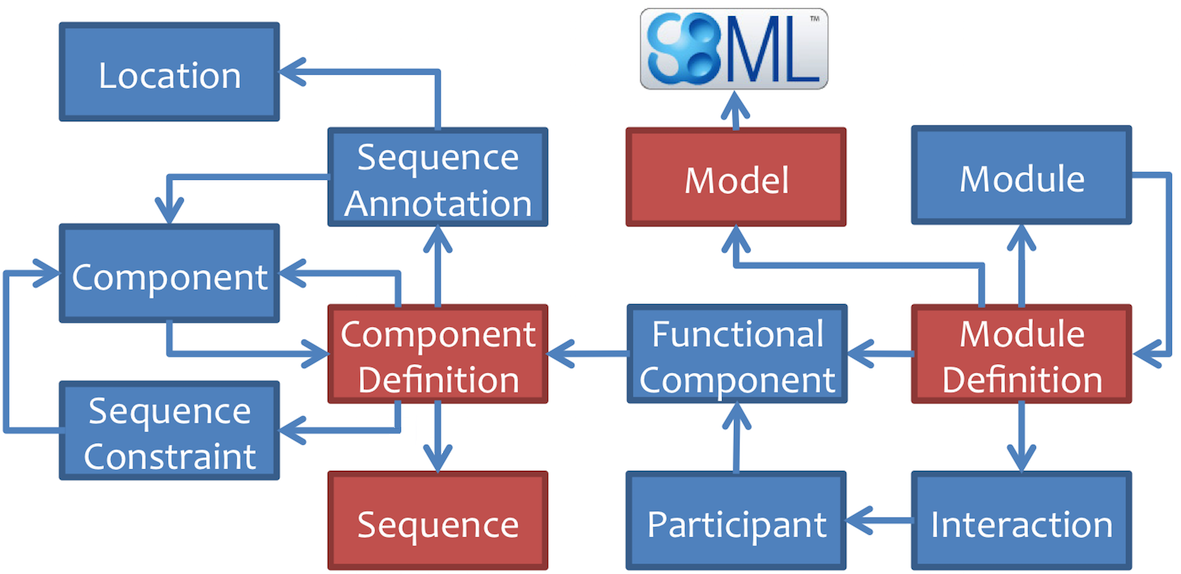
\includegraphics[scale=1.2]{images/SBOL2_2_revised.png}
\caption{Main classes of information represented by the SBOL standard, and their relationships.  Red boxes are ``top level'' classes, while blue classes are used in describing a top-level class; an arrow indicates that one class refers to another.}
\label{images:overview}
\end{center}
\end{figure}
\Rtodo{Put a caption on the figure -JSB  Done -KC Tweaked further -JSB}
\Ctodo{Remove SBML from the figure -JSB, Why?  We have done more with SBML than any alternative?  We already have SBOL2 to SBML and SBML to SBOL2, for example. - CJM}

The \sbol{Sequence} is a fundamental information object for synthetic biology and is needed to reuse components, to replicate synthetic biology work, and to assemble new synthetic biological systems. In designed systems such objects can consist of small chemical molecules, DNAs, RNAs or Proteins. The \sbol{Sequence} object has been designed to encapsulate any of these types of molecules. Small molecule \sbol{Sequence} objects are typically referred to via their chemical formulae. Molecules where sequence specific information is important, such as DNA, RNA and Protein \sbol{Sequence} objects, use the object to incorporate this information. The \sbol{Sequence} object encapsulates this positional information as well as the associated experimental work or other information related to a sequenced molecule.

\Rtodo{need to make it clear that it includes DNA, RNA, and protein, also smooth the text --JSB made addiitons based upon the suggested changes - KC}

In the SBOL data model, a structural layer defines the physical arrangement of components in a biological system.  \sbol{ComponentDefinition}s define genetic elements such as promoters, RBSs, CDSs, and terminators, as well as RNA, proteins, and small molecules.  In a structural hierarchy, \sbol{ComponentDefinition}s can contain subcomponents (\sbol{Component}s), which are instances of the \sbol{ComponentDefinition} for that subcomponent.  A functional layer can be defined to describe the behaviors that arise from the structural layer.  \sbol{ModuleDefinition}s contain information about molecular interactions and their participating components.  They can contain \sbol{FunctionalComponent}s that are instances of \sbol{ComponentDefinition}s that can be assigned functional properties, and they can also contain other modules in a functional hierarchy.  The functions and interactions of these components and other modules within the \sbol{ModuleDefinition} can be quantitatively or qualitatively described using a \sbol{Model}. The \sbol{SequenceAnnotation} object defines data associated the \sbol{Sequence} and \sbol{ComponentDefinition} objects that is needed beyond basic definitions. This can refer to local annotations of the object as well as a container for URIs to external information sources. 


SBOL includes different entities to describe such genetic circuits. Genetic elements such as a promoter, ribosome binding site (RBS), coding sequence (CDS), or terminator are defined with the \sbol{ComponentDefinition} entity. Their instances are reused in different designs via the \sbol{Component}s that refer to corresponding \sbol{ComponentDefinition}s. \sbol{ComponentDefinition}s can also represent proteins, RNAs or small molecules. They are associated with sequence information such as nucleotides aminoacids or chemical structure. A full description of a genetic circuit is then represented using  \sbol{ModuleDefinition}s which contains information about molecular interactions and their participating components. Modules can be associated with quantitative or qualitative models using the \sbol{Model} entity, which is used to point to the actual location of a model. 
\sbol{SequenceAnnotation}s can be used to carry data associated with the successful running of that model on another computer, can be used to point towards sources of some or all of the circuit and the location of experimental data associated with the development of the model.

\Rtodo{Need to also explain annotation --JSB
Provided some text for review describing annotation - KC}



SBOL facilitates the design of complex systems using hierarchical composition. In addition to using simple genetic elements in a modular fashion, modules that are composed of multiple, different components can also be reused. Such modules can expose some of the design components as inputs and outputs, which can be connected to components from other modules using \sbol{MapsTo} entities.


\Ctodo{This needs to be clarified.  Do we really want to explain MapsTo here? -JSB}
\Ctodo{it's not in the diagram. So it should be removed or dealt with in the figure and earlier in the text- KC}

\Ctodo{Explain why it is important to separate definitions from instantiations?}

\LDtodo{The motivation for separating structural and functional considerations is not explained.  Which class names are structural, which class names are functional, and how are the two connected?  Do all structural components require a functional counterpart?  If not, explain why only a subset of structural components would have functional definitions.}

\Ctodo{As a person reading about SBOL2 for the first time, I rank this as the most important section.  While the document should be technically focused overall, this section is your chance to concisely tell someone who won't read the whole document about the take-home messages for the new data model.}

\LDtodo{Why are URI's needed for Components?  Why not just for ComponentDefinitions?  Is there anything in SBOL that does not require a URI?}
\Ctodo{Also briefly mention URI}

\Ctodo{Make sure we explain about annotations up in the motivation and overview, since it's really, really important.}

% The same toggle switch is now displayed using two LacI and TetR inverter submodules in figure \ref{images:toggleswitch_modular}. The LacI inverter uses LacI as input and produces the TetR output, and the TetR inverter uses TetR as input and produces the LacI output. These inputs and outputs are mapped in a parent module.

% Removed as redundant:
%-----------------------------------------------------------------------------
%\section{Introduction}
% -----------------------------------------------------------------------------
%While the first version of the Synthetic Biology Open Language (SBOL) has been adopted by several academic and commercial genetic design automation (GDA) software tools, it only covers a limited range of the requirements for a standardized exchange format for synthetic biology. The SBOL 2.0 specification revises version 1.1, enabling the representation of a wider range of components with and without sequences, including RNA components, protein components, small molecules, and molecular complexes. Additionally, the latest SBOL can be used to convey the intended function of a design, as well as its structural composition. 
%This dichotomous representation of the structural and functional features of a design is a paradigm applied to great success in electrical and computer engineering, and is essential for the development of design automation software in synthetic biology.
%
%The goal of this specification is to define the terminology and relationships used to describe biological designs. In order to provide a shared understanding between engineers seeking to exchange biological designs, SBOL provides a common definition of the concepts needed. As much as possible, we attempt to make explicit the meaning of all terminology and data structures.


% % -----------------------------------------------------------------------------
% \section{Overview of SBOL}
% % -----------------------------------------------------------------------------
% Typically, information about a  genetic circuit includes the order of its constituents and their descriptions. The exact locations of these constituents and their sequences allow genetic circuits to be defined unambiguously, and reused in other designs. Interactions between these constituents are then used to construct biologically plausible designs. 

% In the figure below, a simple toggle switch system is displayed, in which LacI and TetR repress each other's genes transcriptionally. The toggling of the system  is controlled by adding IPTG to deactivate LacI, and ATC to deactivate TetR. The components of the system includes genetic elements, proteins, small molecules.

% \begin{figure}[ht]
% \begin{center}
% 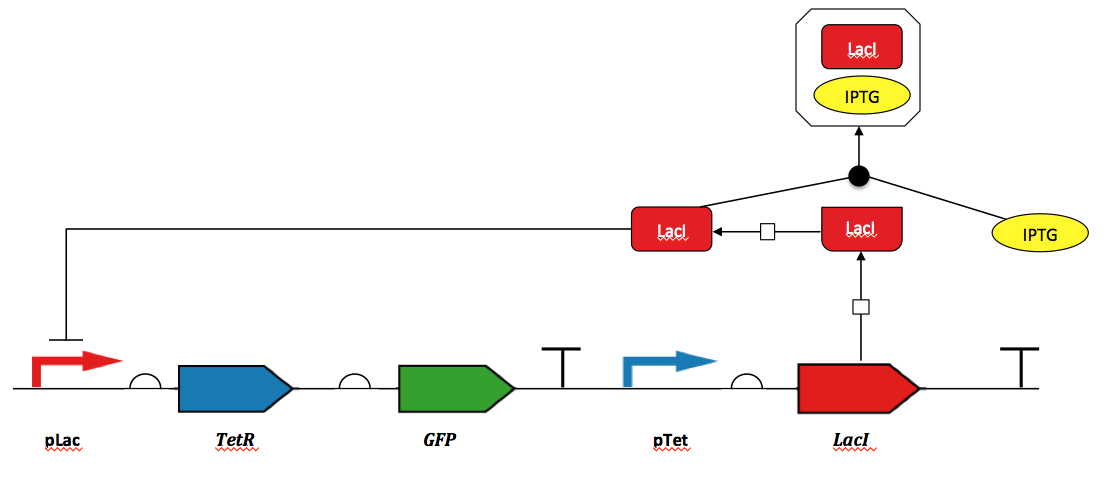
\includegraphics[scale=0.4]{images/toggleswitch_flat}
% \caption[]{An example toggle swicth genetic circuit. }
% \label{images:toggleswitch_flat}
% \end{center}
% \end{figure}

% SBOL includes different entities to describe such genetic circuits. Genetic elements such as promoters, RBS, CDSs and terminators are defined with the \sbol{ComponentDefinition} entity. Their instances are reused in different designs via the \sbol{Component}s that refer to corresponding \sbol{ComponentDefinition}s. \sbol{ComponentDefinition}s can also represent proteins, RNAs or small molecules. They are associated with sequence information such as nucleotides aminoacids or chemical structure. A full description of a genetic circuit is then represented using  \sbol{ModuleDefinition}s which contains information about molecular interactions and their participating components. Modules can be associated with quantitative or qualitative models using the \sbol{Model} entity, which is used to point to the actual location of a model.


% SBOL facilitates the design of complex systems using hierarchical composition. In addition to using simple genetic elements in a modular fashion, modules that are composed of multiple, different components can also be reused. Such modules can expose some of the design components as inputs and outputs, which can be connected to components from other modules using \sbol{MapsTo} entities.